\documentclass[12pt,a4paper,bahasa]{article}
\usepackage{graphicx}


\begin{document}

\title{ANALISIS PROSES BISNIS KTP}
\maketitle

\textbf{SKartu Tanda Penduduk (KTP)} merupakan suatu identitas penduduk (identitas pribadi) yang diterbitkan oleh instansi pelaksana. Kartu ini wajib dimiliki oleh WNI dan WNA yang memiliki izin menetap yang sudah berumur 17 tahun/menikah/sudah pernah menikah.\\

\textbf{Adapun proses bisnis dari KTP adalah:}

\begin {enumerate}

\item Kelurahan mendapat pemberitahuan bahwa warganya diwajibkan membuat KTP lalu kelurahan menginfokan kepada RT/RW bersangkutan.
\item RT/RW memberitahukan info tersebut kepada warganya dan memberikan surat pengantar.
\item Warga meminta tanda tangan/izin dari RT/RW setempat.
\item Warga pergi ke kantor kelurahan/kecamatan.
\item Warga mengambil nomer antrian dan menuju loker verifikasi data diri.
\item Warga mengisi formulir dan petugas melakukan verifikasi data.
\item Warga melakukan perekaman ttd, sidik jari, dan retina mata.
\item Petugas mengambil foto warga untuk pembuatan KTP.
\item Petugas memberitahu warga bahwa ktp sedang dalam proses pembuatan dan akan jadi beberapa hari/minggu lagi.
\item Warga mendapatkan KTP

sudah berumur 17 tahun/menikah/sudah pernah menikah.

\end{enumerate}
\textbf{Adapun proses bisnis dari KTP adalah:}\\
\textbf{Atribut (universal) yang dimiliki oleh KTP adalah:}\\
\begin{enumerate}

\item NIK
\item Nama
\item Tempat/Tgl lahir
\item Jenis Kelamin
\item Alamat
\item RT/.RW
\item Kel/Desa
\item Kecamatan
\item Agama
\item Status Perkawinan
\item Pekerjaan
\item Kewarganegaraan
\item Berlaku Hingga
\item Foto
\item Tanda Tangan
\item Provinsi
\item Kabupaten
\item Tanggal pembuatan
\end{enumerate}

\begin{enumerate}


\item Tabel RT/RW\\
\begin{figure}[!htbp]
\centering
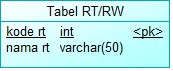
\includegraphics[scale=1.0]{gambar/Rt.jpeg}
\caption{\textit{RT/RW}}
\label{RT/RW}
\end{figure}
Atribut asli pada tabel RT/RW adalah:\\
•	Kode RT/RW \\
•	Nama RT/RW\\
Primary Key pada tabel RT/RW:\\
•	Kode RT

\item Tabel Kelurahan\\
\begin{figure}[!htbp]
\centering
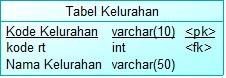
\includegraphics[scale=1.0]{gambar/Kelurahan.jpeg}
\caption{\textit{Kelurahan}}
\label{Kelurahan}
\end{figure}
Atribut asli pada tabel Kelurahan:\\
•	Kode Kelurahan\\
•	Nama Kelurahan\\
Primary Key pada tabel Kelurahan:\\
•	Kode kelurahan\\
Foreign Key pada tabel kelurahan:\\
•	Kode RT

\item Tabel Kecamatan\\
\begin{figure}[!htbp]
\centering
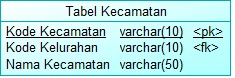
\includegraphics[scale=1.0]{gambar/Kecamatan.jpeg}
\caption{\textit{Kecamatan}}
\label{Kecamatan}
\end{figure}
Atribut asli pada tabel Kecamatan:\\
•	Kode Kecamatan\\
•	Nama Kecamatan\\
Primary Key:\\
•	Kode Kecamatan\\
Foreign Key:\\
•	Kode Kelurahan

\item Tabel Kota\\
\begin{figure}[!htbp]
\centering
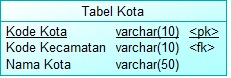
\includegraphics[scale=1.0]{gambar/Kota.jpeg}
\caption{\textit{Kota}}
\label{Kota}
\end{figure}
Atribut asli pada tabel Provinsi:\\
•	Kode Kota\\
•	Nama Kota\\
Primary Key:\\
•	Kode Kota\\
Foreign Key:\\
•	Kode Kecamatan

\item Tabel Provinsi\\
\begin{figure}[!htbp]
\centering
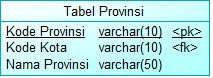
\includegraphics[scale=1.0]{gambar/Provinsi.jpeg}
\caption{\textit{Provinsi}}
\label{Provinsi}
\end{figure}
Atribut asli pada tabel Provinsi:\\ 
•	Kode Provinsi\\
•	Nama Provinsi\\
Primary Key:\\
•	Kode Provinsi\\
Foreign Key:\\
•	Kode Kota
\\
\\
\\
\\
\\
\\
\item Tabel Kewarganegaraan\\
\begin{figure}[!htbp]
\centering
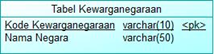
\includegraphics[scale=0.8]{gambar/Kewarganegaraan.png}
\caption{\textit{Kewarganegaraan}}
\label{Kewarganegaraan}
\end{figure}
Atribut asli pada tabel Kewarganegaraan:\\
•	Kode kewarganegaraan\\
•	Nama negara \\
Primary Key:\\
•	Kode kewarganegaraan

\item Tabel Pekerjaan\\
\begin{figure}[!htbp]
\centering
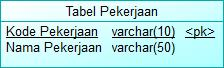
\includegraphics[scale=1.0]{gambar/Pekerjaan.jpeg}
\caption{\textit{Pekerjaan}}
\label{Pekerjaan}
\end{figure}
Atribut asli pada tabel Pekerjaan:\\
•	Kode Pekerjaan\\
•	Nama Pekerjaan\\
Primary Key:\\
•	Kode Pekerjaan

\item Tabel Perkawinan\\
\begin{figure}[!htbp]
\centering
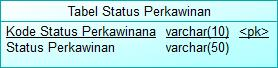
\includegraphics[scale=1.0]{gambar/Perkawinan.jpeg}
\caption{\textit{Perkawinan}}
\label{Perkawinan}
\end{figure}
Atribut asli pada tabel Status Perkawinan:\\ 
•	Kode Status Perkawinan\\
•	Status Perkawinan\\
Primary Key:\\
•	Kode Status Perkawinan
\\
\\
\item Tabel Agama\\
\begin{figure}[!htbp]
\centering
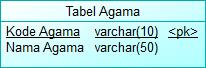
\includegraphics[scale=1.0]{gambar/Agama.jpeg}
\caption{\textit{Agama}}
\label{Agama}
\end{figure}
Atribut asli pada tabel Agama:\\
•	Kode Agama\\
•	Nama Agama\\ 
Primary Key:\\
•	Kode Agama

\item Tabel Jenis Kelamin\\
\begin{figure}[!htbp]
\centering
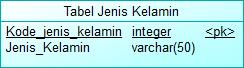
\includegraphics[scale=1.0]{gambar/JenisKelamin.jpeg}
\caption{\textit{Jenis Kelamin}}
\label{Jenis Kelamin}
\end{figure}
Atribut asli pada tabel Jenis Kelamin:\\
•	Kode Jenis Kelamin\\
•	Jenis Kelamin\\
Primary Key:\\
•	Kode Jenis Kelamin

\item Tabel Golongan Darah\\
\begin{figure}[!htbp]
\centering
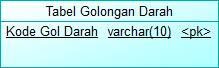
\includegraphics[scale=1.0]{gambar/Goldar.jpeg}
\caption{\textit{Golongan Darah}}
\label{Golongan Darah}
\end{figure}
Atribut asli dan Primary Key pada tabel Golongan Darah\\
•	Kode Gol Darah
\\
\\
\\
\\
\\
\item Tabel Pengesahan\\
\begin{figure}[!htbp]
\centering
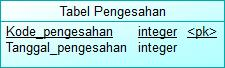
\includegraphics[scale=1.0]{gambar/Pengesahan.jpeg}
\caption{\textit{Pengesahan}}
\label{Pengesahan}
\end{figure}
Atribut asli dan Primary Key pada tabel Pengesahan:\\
•	Kode Pengesahan\\
•	Tanggal Pengesahan

\item Tabel Penduduk\\
\begin{figure}[!htbp]
\centering
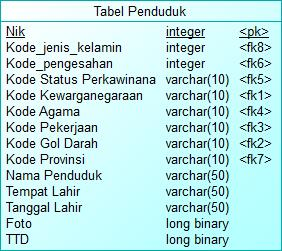
\includegraphics[scale=0.8]{gambar/Penduduk.jpeg}
\caption{\textit{Penduduk}}
\label{Penduduk}
\end{figure}
Adapun Atribut asli pada tabel Penduduk adalah:\\
•	Nik\\
•	Nama Penduduk\\
•	Tempat Lahir\\
•	Tanggal Lahir\\
•	Foto\\
•	TTD\\
Primary Key:\\
•	NIK\\
Foreign Key:\\
•	Kode jenis kelamin\\
•	Kode pengesahan\\
•	Kode status perkawinan\\
•	Kode kewarganegaraan\\
•	Kode agama\\
•	Kode pekerjaan\\
•	Kode gol darah\\
•	Kode provinsi\\
\\
Pyscical Data Modeling 
\end{enumerate}
\begin{figure}[!htbp]
\centering
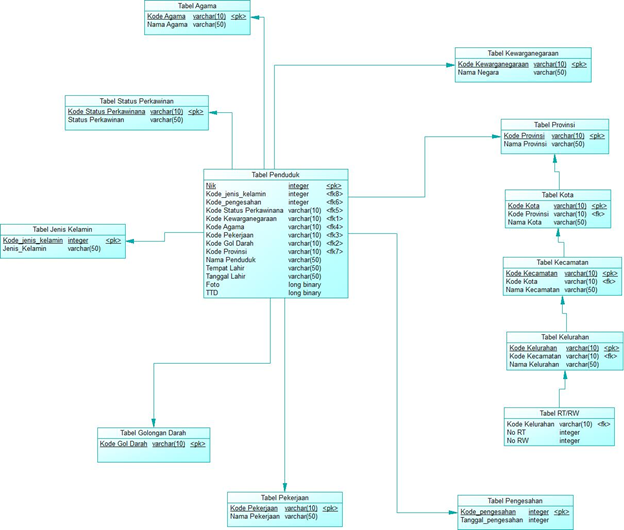
\includegraphics[scale=0.8]{gambar/Pdm.png}
\caption{\textit{Pdm}}
\label{Pdm}
\end{figure}

\textbf{CARDINALITAS}
\begin{enumerate}
\item Relasi antara tabel RT/RW dengan tabel Kelurahan (many-one)
Satu kelurahan membutuhkan/terdiri dari banyak RT/RW. 
\item Relasi antara tabel Kelurahan dengan Kecamatan (many-one)
Satu kecamatan membutuhkan/terdiri dari banyak kelurahan. 
\item Relasi antara tabel kecamatan dengan kota (many-one)
Satu kota membutuhkan/terdiri dari banyak kecamatan.
\item Relasi antara tabel kota dengan provinsi (many-one)
Satu provinsi membutuhkan/terdiri dari banyak kota.
\item Relasi antara tabel penduduk dengan provinsi dengan penduduk (one-many)
Banyak penduduk membutuhkan/terdiri dari satu provinsi.
\item Relasi antara tabel penduduk dengan pengesahan  (one-many)
Banyak penduduk membutuhkan/terdiri satu pengesahan.
\item Relasi antara tabel penduduk dengan pekerjaan (one-many)
Banyak penduduk membutuhkan/terdiri satu pekerjaan.
\item Relasi antara tabel penduduk dengan golongan darah (one-many)
Banyak penduduk membutuhkan/terdiri satu golongan darah.
\item Relasi antara tabel penduduk dengan jenis kelamin (one-many)
Banyak penduduk membutuhkan/terdiri satu jenis kelamin.
\item Relasi antara tabel penduduk dengan agama (one-many)
Banyak penduduk membutuhkan/terdiri satu agama.
\item Relasi antara tabel penduduk dengan kewarganegaraan (one-many)
Banyak penduduk membutuhkan/terdiri satu kewarganegaraan.
\item Relasi antara tabel penduduk dengan status perkawinan (one-many)
Banyak penduduk membutuhkan/terdiri satu status perkawinan.
\\\\\\\\
\\\\\\\\
\\\\\\\\
\\\\\\\\
\\\\\\\\
\end{enumerate}
\textbf{Conceptual  Data Modeling}

\begin{figure}[!htbp]
\centering
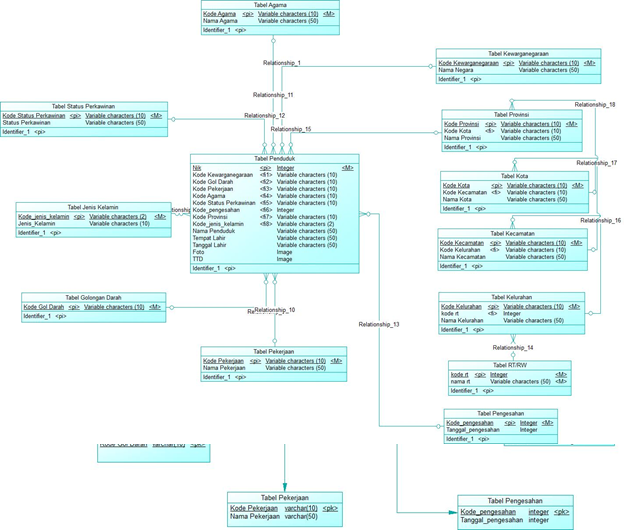
\includegraphics[scale=0.8]{gambar/Cdm.png}
\caption{\textit{Cdm}}
\label{Cdm}
\end{figure}
\textbf{Note: mandatory dimaksud agar saat pengisian atribut tidak bernilai kosong (null)}
\end{document}